\documentclass[10pt]{article}
\usepackage[margin=0.8in]{geometry}
\usepackage[utf8]{inputenc}
\usepackage[T1]{fontenc}
\usepackage{graphicx}
\usepackage[export]{adjustbox}
\usepackage{amsmath}
\usepackage{amsfonts}
\usepackage{amssymb}
\usepackage[version=4]{mhchem}
\usepackage{stmaryrd}
\usepackage{bbold}
\usepackage{fixltx2e}
\usepackage{caption}
\usepackage{mathtools}
\usepackage[parfill]{parskip}
\usepackage{float}
\usepackage{amsmath}

\usepackage[framemethod=TikZ]{mdframed}
\colorlet{shadecolor}{orange!15}
\usepackage{xcolor}
\usepackage{amsthm}
\usepackage{framed}

\begin{document}


\title{Lecture 22: Operational Space Control}
\author{Wanxin Jin}
\maketitle



% \subsection{General Schemes}
% As pointed out above, operational space control schemes are based on a direct comparison of the inputs, specifying operational space trajectories, with the measurements of the corresponding manipulator outputs. It follows that the control system should incorporate some actions that allow the transformation from the operational space, in which the error is specified, to the joint space, in which control generalized forces are developed.

% A possible control scheme that can be devised is the so-called Jacobian inverse control. In this scheme, the end-effector pose in the operational space $\boldsymbol{x}_{e}$ is compared with the corresponding desired quantity $\boldsymbol{x}_{d}$ and then an operational space deviation $\Delta \boldsymbol{x}$ can be computed. Assumed that this deviation is sufficiently small for a good control system, $\Delta \boldsymbol{x}$ can be transformed into a corresponding joint space deviation $\Delta \boldsymbol{q}$ through the inverse of the manipulator Jacobian. Then, the control input generalized forces can be computed on the basis of this deviation through a suitable feedback matrix gain. The result is a presumable reduction of $\Delta \boldsymbol{q}$ and in turn of $\Delta \boldsymbol{x}$. In other words, the Jacobian inverse control leads to an overall system that intuitively

% \begin{figure} [H]
%     \centering
%     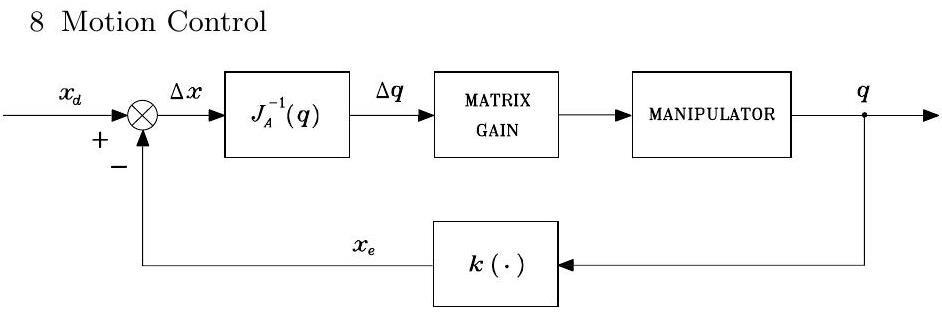
\includegraphics[max width=0.5\textwidth]{control/jacobian_inverse_control.jpg}
%     \caption{Block scheme of Jacobian inverse control}
%     \label{fig:enter-label}
% \end{figure}

% \begin{figure} [H]
%     \centering
%     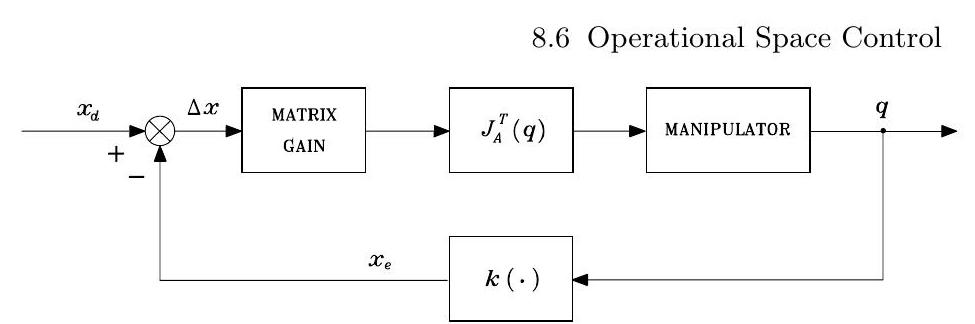
\includegraphics[max width=0.5\textwidth]{control/jacobian_transpose_control.jpg}
%     \caption{Block scheme of Jacobian transpose control}
%     \label{fig:enter-label}
% \end{figure}





% behaves like a mechanical system with a generalized $n$-dimensional spring in the joint space, whose constant stiffness is determined by the feedback matrix gain. The role of such system is to take the deviation $\Delta \boldsymbol{q}$ to zero. If the matrix gain is diagonal, the generalized spring corresponds to $n$ independent elastic elements, one for each joint.

% A conceptually analogous scheme is the so-called Jacobian transpose control. In this case, the operational space error is treated first through a matrix gain. The output of this block can then be considered as the elastic force generated by a generalized spring whose function in the operational space is that to reduce or to cancel the position deviation $\Delta \boldsymbol{x}$. In other words, the resulting force drives the end-effector along a direction to reduce $\boldsymbol{\Delta} \boldsymbol{x}$. This operational space force has then to be transformed into the joint space generalized forces, through the transpose of the Jacobian, to realize the described behavior.

% Both Jacobian inverse and transpose control schemes have been derived in an intuitive fashion. Hence, there is no guarantee that such schemes are effective in terms of stability and trajectory tracking accuracy. These problems can be faced by presenting two mathematical solutions below, which will be shown to be substantially equivalent to the above schemes.


If the motion $\boldsymbol{x}_d$ is specified in the operational space, the  joint  variable $\boldsymbol{q}$ can be transformed into the  operational space variables through forward kinematics: $\boldsymbol{x}_e=\boldsymbol{k}(\boldsymbol{q})$. Then, the operational space error
\begin{equation}\label{equ.end_pose_error}
    \boldsymbol{e}=\boldsymbol{x}_d-\boldsymbol{x}_e
\end{equation}
allows the design of  control that uses the feedback from the error operation space.



In the following control design for a $n$-joint manipulator, we consider a manipulator without external end-effector forces  and  any joint friction.   The equation of motion of the manipulator thus is 

\begin{equation}\label{equ.manipulator}
    \boldsymbol{B}(\boldsymbol{q}) \ddot{\boldsymbol{q}}+\boldsymbol{C}(\boldsymbol{q}, \dot{\boldsymbol{q}}) \dot{\boldsymbol{q}}+\boldsymbol{g}(\boldsymbol{q})=\boldsymbol{u}
\end{equation}

The controller we want to design is in the general form of 
\begin{equation}\label{equ.controller}
\boldsymbol{u}=\textbf{Controller}(\boldsymbol{q}, \boldsymbol{\dot{q}}, \boldsymbol{x}_d, \boldsymbol{\dot{x}}_d)
\end{equation}
i.e., the controller takes as input the manipulator's current joint position $\boldsymbol{q}$, current joint velocity $\boldsymbol{\dot{q}}$, the desired end-effector pose $\boldsymbol{x}_d$, and desired end-effector velocity $\boldsymbol{\dot{x}}_d$, and outputs the joint torque $\boldsymbol{u}$.

Thus, the controlled manipulator  with the controller  is 
\begin{equation}\label{equ.manipulator_control}
    \boldsymbol{B}(\boldsymbol{q}) \ddot{\boldsymbol{q}}+\boldsymbol{C}(\boldsymbol{q}, \dot{\boldsymbol{q}}) \dot{\boldsymbol{q}}+\boldsymbol{g}(\boldsymbol{q})=\textbf{Controller}(\boldsymbol{q}, \boldsymbol{\dot{q}}, \boldsymbol{x}_d, \boldsymbol{\dot{x}}_d)
\end{equation}



By analogy with joint space centralized control, we below will consider two types of  controllers for the operational space control.


\section{Controller I: PD Control with Gravity Compensation}
Given a constant end-effector pose $\boldsymbol{x}_{d}$, one can define the pose error of the end-effector as in (\ref{equ.end_pose_error}). We want to design a controller (\ref{equ.controller}), such that from  any initial configuration, say $\boldsymbol{q}_0$, the controlled manipulator (\ref{equ.manipulator_control}) will eventually reach $\boldsymbol{x}_{d}$. That means  the end-effector error in (\ref{equ.end_pose_error}) has
$$
\boldsymbol{e}(t)\rightarrow \boldsymbol{0}\quad \text{as}\quad
t\rightarrow \infty
$$

Below, we will design the controller (\ref{equ.controller}) based on the Lyapunov method (see  background of Lyapunov method in Lecture 16-17). First, we take the vector $\begin{bmatrix}\boldsymbol{e}\\
\boldsymbol{\dot{q}}\end{bmatrix}$  as the control system state. Choose the following positive definite quadratic form as Lyapunov function candidate:

$$
V(\dot{\boldsymbol{q}}, {\boldsymbol{e}})=\frac{1}{2} \dot{\boldsymbol{q}}^{T} \boldsymbol{B}(\boldsymbol{q}) \dot{\boldsymbol{q}}+\frac{1}{2} {\boldsymbol{e}}^{T} \boldsymbol{K}_{P} {\boldsymbol{e}}>0 \quad \forall \dot{\boldsymbol{q}}, {\boldsymbol{e}} \neq \mathbf{0}
$$

with $\boldsymbol{K}_{P}$ a symmetric positive definite matrix. Then,

$$
\dot{V}=\dot{\boldsymbol{q}}^{T} \boldsymbol{B}(\boldsymbol{q}) \ddot{\boldsymbol{q}}+\frac{1}{2} \dot{\boldsymbol{q}}^{T} \dot{\boldsymbol{B}}(\boldsymbol{q}) \dot{\boldsymbol{q}}+\dot{\boldsymbol{e}}^{T} \boldsymbol{K}_{P} {\boldsymbol{e}}
$$

\begin{figure}[H]
    \centering
    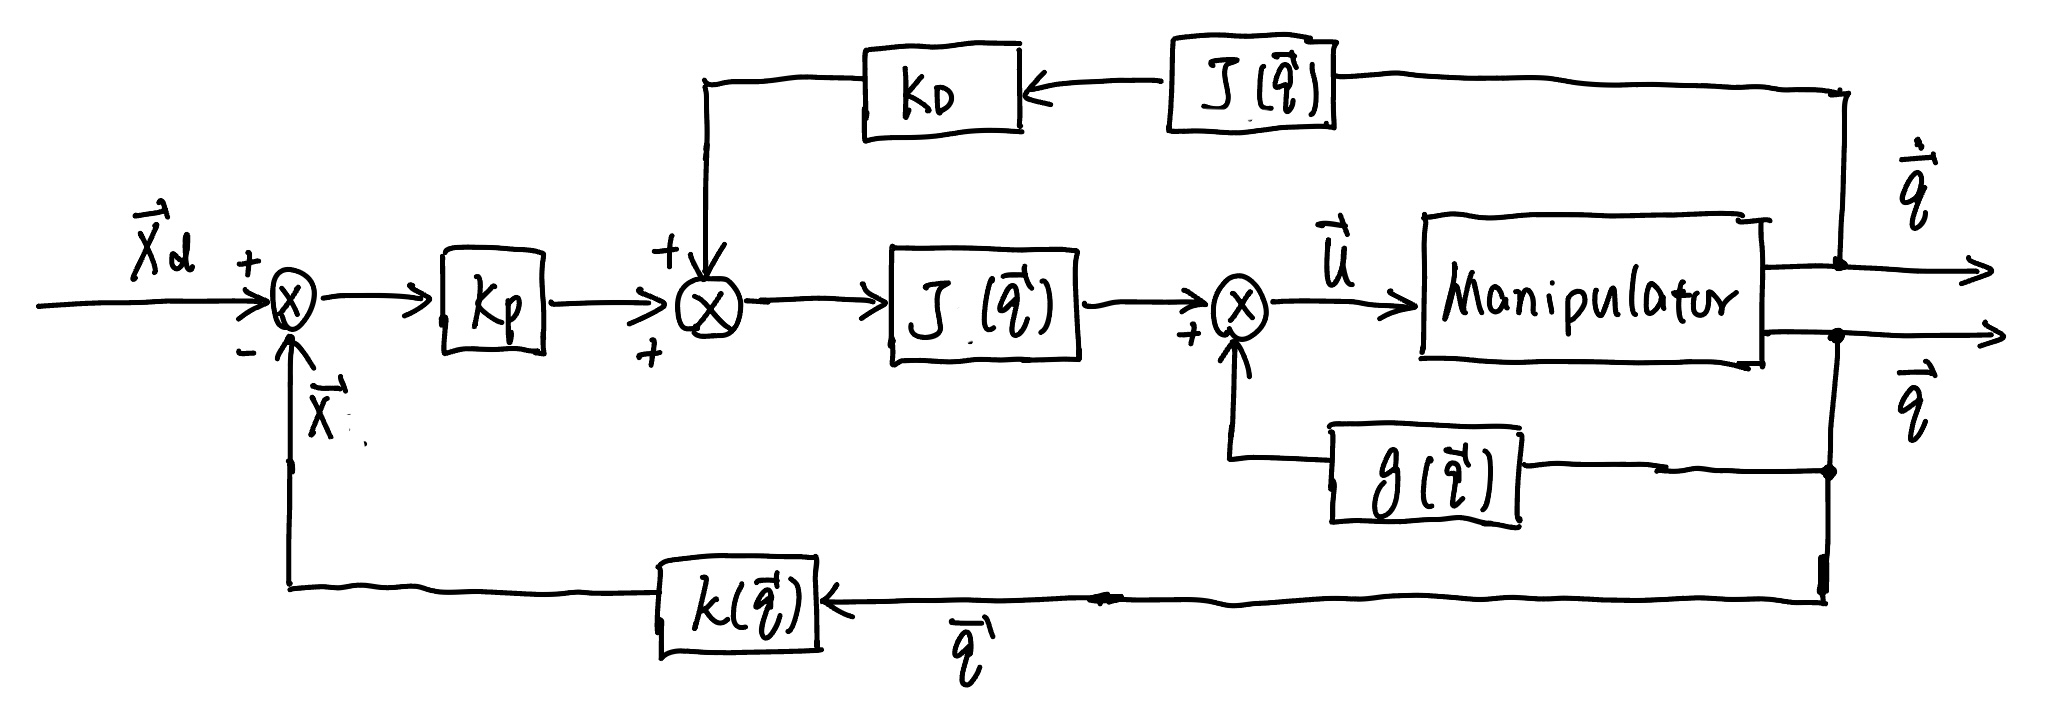
\includegraphics[max width=0.60\textwidth]{control/operational_PD_gravity_compensation.jpeg}
    \caption{Block diagram of operational space PD control with gravity compensation}
    \label{fig:3}
\end{figure}


Since $\dot{\boldsymbol{x}}_{d}=\mathbf{0}$, 

$$
\dot{{\boldsymbol{e}}}=-\boldsymbol{J}_{A}(\boldsymbol{q}) \dot{\boldsymbol{q}}
$$

and then

$$
\dot{V}=\dot{\boldsymbol{q}}^{T} \boldsymbol{B}(\boldsymbol{q}) \ddot{\boldsymbol{q}}+\frac{1}{2} \dot{\boldsymbol{q}}^{T} \dot{\boldsymbol{B}}(\boldsymbol{q}) \dot{\boldsymbol{q}}-\dot{\boldsymbol{q}}^{T} \boldsymbol{J}_{A}^{T}(\boldsymbol{q}) \boldsymbol{K}_{P} {\boldsymbol{e}}
$$

Similar to the derivation in the previous lecture, we replace $\boldsymbol{B}\ddot{\boldsymbol{q}}$ form dynamics (\ref{equ.manipulator}) and consider the property that $\boldsymbol{N}=\dot{\boldsymbol{B}}-2 \boldsymbol{C}$ is a skew-symmetric matrix (see in the property of dynamics in Lecture 18). Then, the time derivative of Lyapunov function is 

$$
\dot{V}=\dot{\boldsymbol{q}}^{T}\left(\boldsymbol{u}-\boldsymbol{g}(\boldsymbol{q})-\boldsymbol{J}_{A}^{T}(\boldsymbol{q}) \boldsymbol{K}_{P} {\boldsymbol{e}}\right) .
$$

For the above $\dot{V}$ to be negative, we choose the controller
\begin{shaded}
\begin{equation}
        \boldsymbol{u}=\boldsymbol{g}(\boldsymbol{q})+\boldsymbol{J}_{A}^{T}(\boldsymbol{q}) \boldsymbol{K}_{P} {\boldsymbol{e}}-\boldsymbol{J}_{A}^{T}(\boldsymbol{q}) \boldsymbol{K}_{D} \boldsymbol{J}_{A}(\boldsymbol{q}) \dot{\boldsymbol{q}}
\end{equation}
\end{shaded}
with $\boldsymbol{K}_{D}$ positive definite, then,
$$
\dot{V}=-\dot{\boldsymbol{q}}^{T} \boldsymbol{J}_{A}^{T}(\boldsymbol{q}) \boldsymbol{K}_{D} \boldsymbol{J}_{A}(\boldsymbol{q}) \dot{\boldsymbol{q}} \quad <0,  \quad \forall \quad\boldsymbol{\dot{q}}\quad\text{with} \quad \boldsymbol{J}_A(\boldsymbol{q})\dot{\boldsymbol{q}} \neq \mathbf{0}
$$
which says  the Lyapunov function decreases as long as $\boldsymbol{J}_A(\boldsymbol{q})\dot{\boldsymbol{q}} \neq \mathbf{0}$. Thus, the system reaches an   equilibrium pose, with condition $\dot{V}= 0$ and $\boldsymbol{J}_A(\boldsymbol{q})\dot{\boldsymbol{q}}=\mathbf{0}$. We consider the non-redundant non-singularity of matrix $\boldsymbol{J}_A(\boldsymbol{q})$. Then, the equilibrium condition $\boldsymbol{J}_A(\boldsymbol{q})\dot{\boldsymbol{q}}=\mathbf{0}$ means that $\dot{\boldsymbol{q}}=\mathbf{0}$ and further $\ddot{\boldsymbol{q}} =\mathbf{0}$.



To find the equilibrium configuration, we look at the manipulator dynamics under control

$$
\boldsymbol{B}(\boldsymbol{q}) \ddot{\boldsymbol{q}}+\boldsymbol{C}(\boldsymbol{q}, \dot{\boldsymbol{q}}) \dot{\boldsymbol{q}}+\boldsymbol{F} \dot{\boldsymbol{q}}+\boldsymbol{g}(\boldsymbol{q})=\boldsymbol{g}(\boldsymbol{q})+\boldsymbol{J}_{A}^{T}(\boldsymbol{q}) \boldsymbol{K}_{P} {\boldsymbol{e}}-\boldsymbol{J}_{A}^{T}(\boldsymbol{q}) \boldsymbol{K}_{D} \boldsymbol{J}_{A}(\boldsymbol{q}) \dot{\boldsymbol{q}}
$$

With the condition  $\dot{\boldsymbol{q}}=\mathbf{0}$, it follows that   $\ddot{\boldsymbol{q}} =\mathbf{0}$, and then from the above dynamics, 
$$
\boldsymbol{J}_{A}^{T}(\boldsymbol{q}) \boldsymbol{K}_{P} {\boldsymbol{e}}=\mathbf{0}\quad \rightarrow\quad {\boldsymbol{e}}=\boldsymbol{x}_{d}-\boldsymbol{x}_{e}=\mathbf{0}
$$
This concludes that the controlled manipulator will asymptotically reach $\boldsymbol{x}_d$.
The  control scheme is  in  Fig.  \ref{fig:3}. 

\section{Controller II: Inverse Dynamics Control}
Recall the joint space inverse dynamics control of a manipulator in the previous lecture (Lecture 21), we set the controller of the following form
\begin{shaded}
    \begin{equation}\label{equ:u}
    \boldsymbol{u}=\boldsymbol{B}(\boldsymbol{q}) \boldsymbol{y}+\boldsymbol{C}(\boldsymbol{q}, \dot{\boldsymbol{q}}) \dot{\boldsymbol{q}}+\boldsymbol{g}(\boldsymbol{q})
\end{equation}
\end{shaded}
where $\boldsymbol{y}$ is a new input vector whose expression is to be determined yet. The above controller directly leads to the controlled manipulator (\ref{equ.manipulator_control}) as
$$
 \boldsymbol{B}(\boldsymbol{q}) \ddot{\boldsymbol{q}}+\boldsymbol{C}(\boldsymbol{q}, \dot{\boldsymbol{q}}) \dot{\boldsymbol{q}}+\boldsymbol{g}(\boldsymbol{q})=\boldsymbol{B}(\boldsymbol{q}) \boldsymbol{y}+\boldsymbol{C}(\boldsymbol{q}, \dot{\boldsymbol{q}}) \dot{\boldsymbol{q}}+\boldsymbol{g}(\boldsymbol{q})
 $$
leading to 
\begin{equation}\label{equ.dyn_new}
\boldsymbol{\ddot{q}}=\boldsymbol{y} 
\end{equation}
Again, we will discuss how to set this new control input vector $\boldsymbol{y}$, but the particular form of controller (\ref{equ:u}) leads to a linear relationship between the input signal $\boldsymbol{y}$ and the manipulator's joint acceleration $\ddot{\boldsymbol{q}}$. 



The new control input $\boldsymbol{y}$ in (\ref{equ:u}) is to be designed to track a changing $\boldsymbol{x}_{d}(t)$. To this end, we differentiate the jacobian equation 
$$
\dot{\boldsymbol{x}}_e=\boldsymbol{J}_A(\boldsymbol{q})\dot{\boldsymbol{q}}
$$
on both side with respect to time $t$, leading to 
\begin{equation}\label{equ.dotjacobian}
    \ddot{\boldsymbol{x}}_{e}=\boldsymbol{J}_{A}(\boldsymbol{q}) \ddot{\boldsymbol{q}}+\dot{\boldsymbol{J}}_{A}(\boldsymbol{q}, \dot{\boldsymbol{q}}) \dot{\boldsymbol{q}}
\end{equation}



For a nonredundant manipulator, the above (\ref{equ.dotjacobian}) suggests the following choice of $\boldsymbol{y}$:
\begin{shaded}
    \begin{equation}\label{equ.ysignal}
    \boldsymbol{y}=\boldsymbol{J}_{A}^{-1}(\boldsymbol{q})\left(\ddot{\boldsymbol{x}}_{d}+\boldsymbol{K}_{D} \dot{{\boldsymbol{e}}}+\boldsymbol{K}_{P} {\boldsymbol{e}}-\dot{\boldsymbol{J}}_{A}(\boldsymbol{q}, \dot{\boldsymbol{q}}) \dot{\boldsymbol{q}}\right)
\end{equation}
\end{shaded}
with $\boldsymbol{K}_{P}$ and $\boldsymbol{K}_{D}$ positive definite  matrices. In fact, plugging (\ref{equ.ysignal}) to (\ref{equ.dyn_new}) leads to the  error dynamics

$$
\ddot{{\boldsymbol{e}}}+\boldsymbol{K}_{D} \dot{{\boldsymbol{e}}}+\boldsymbol{K}_{P} {\boldsymbol{e}}=\mathbf{0}
$$

which describes the operational space error dynamics, with $\boldsymbol{K}_{P}$ and $\boldsymbol{K}_{D}$ determining the error convergence rate to zero, as specified in the previous lecture (Lecture 21). Please see my additional control background note for the response of the second-order system versus the values of  $\boldsymbol{K}_{P}$ and $\boldsymbol{K}_{D}$.



The resulting inverse dynamics control scheme is reported in Fig. \ref{fig:44}. Again in this case, besides $\boldsymbol{x}_{e}$ and $\dot{\boldsymbol{x}}_{e}, \boldsymbol{q}$ and $\dot{\boldsymbol{q}}$ are also to be measured. If measurements of $\boldsymbol{x}_{e}$ and $\dot{\boldsymbol{x}}_{e}$ are indirect, the controller must compute the direct kinematics functions $\boldsymbol{k}(\boldsymbol{q})$ and $\boldsymbol{J}_{A}(\boldsymbol{q})$ on-line.

\begin{figure}[H]
    \centering
    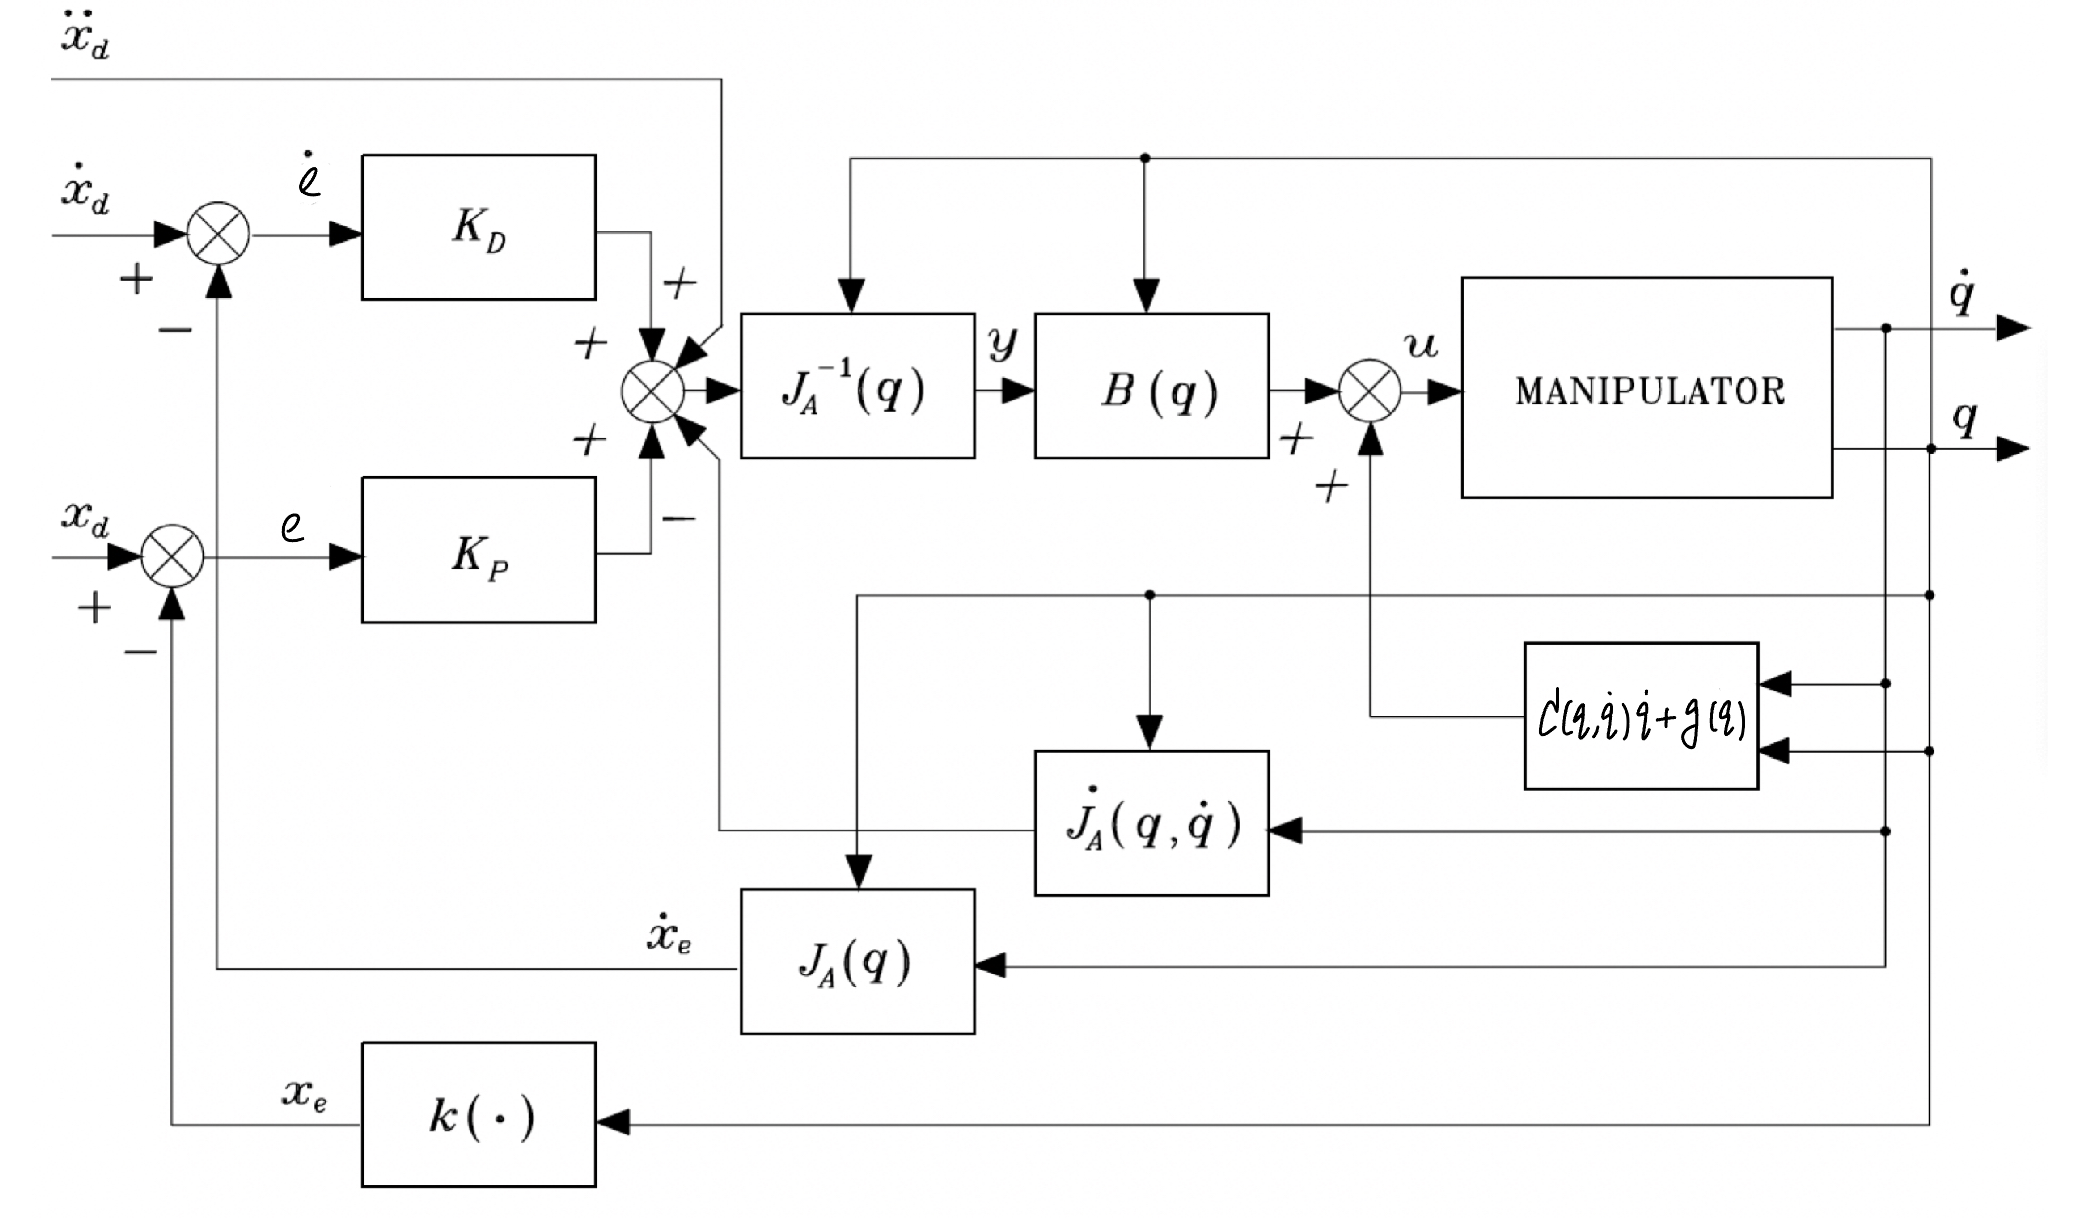
\includegraphics[max width=0.65\textwidth]{control/operational_PD_gravity_compensation2.jpeg}
    \caption{Block scheme of operational space PD control with gravity compensation}
    \label{fig:44}
\end{figure}




\end{document}